\chapter{Visualisierung}
\label{sec:visualisation}

Ziel dieses Kapitels ist es, das erarbeitete Konzept zur Visualisierung der Pain Scores vorzustellen. Das Konzept wird anhand eines Beispielsignals mit einer Aufnahme des Weinenes eines Babys enthält. Das Signal wird in Abbildung \ref{img:visualisation_example_01} oben gezeigt. Der gezeigte Ausschnitt ist insgesamt 220 Sekunden lang. Die Signalabschnitte, die Stimme des Babys enthalten, werden Schwarz dargestellt, das Hintergrundrauschen grau. Das Signal wurde segmentiert mit $t_{s} = \SI{10}{\second}$ und so zwei Segmente gefunden. Die beiden Segmente sind $30.5$ Sekunden voneinander entfernt. Zur Schmerzdiagnostik auf Basis zwei verschiedener fiktiver Pain Scales durchgeführt, welche in Tabelle \ref{tab:fictional_painscales_viz} aufgeführt werden. Die \glqq Length-Scale\grqq{} bewertet den Schmerzgrad nach der Länge des Weinens und vergibt einen maximalen Score on 2, die \glqq Min-Scale\grqq bewertet die Qualität des Weinens und vergibt einen maximalen Score von 3.

\begin{table}[h]
\centering
\caption{Fiktive Pain Scales zur Erläuterung der Visualisierung}
\label{tab:fictional_painscales_viz}
\begin{tabular}{@{}lll@{}}
\toprule
         & \glqq Length-Scale\grqq  & \glqq Min-Scale\grqq        \\ \midrule
0 Punkte & kein Weinen   & Lachen           \\
1 Punkt  & kurzes Weinen & leichtes Weinen  \\
2 Punkte & langes Weinen & mittleres Weinen \\
3 Punkte & -             & starkes weinen   \\ \bottomrule
\end{tabular}
\end{table}

Mit Hilfe einer der in Kapitel \ref{sec:deduction} vorgestellten Strategien wurden Formeln zur Ableitung der Schmerz Scores nach objektiv messbaren Eigenschaften gefunden. Gleichung \ref{eq:ps_length} definiert die Funktion $PS_{Length}$, welche die Pain Score für Segmente nach der \glqq Length-Scale\grqq{} ableitet. Aus der Gleichung geht hervor, dass ein Pain Score von 0 für ein Segment nicht abgeleitet werden kann, da die Anwesenheit eines Segmentes der Abwesenheit von Weinen implizit widerspricht. Gleichung  \ref{eq:ps_length} definiert die Funktion $PS_{Max}$ zur Schmerzableitung nach der \glqq Min-Scale\grqq. 
\begin{equation}
PS_{Length}(cs) = \begin{cases}
 1 \quad ,  \text{wenn } \text{S-Length}(cs) \leq \SI{1}{\minute} \\
 2 \quad ,  \text{wenn } \text{S-Length}(cs) > \SI{1}{\minute}
 \end{cases}	
 \label{eq:ps_length}
\end{equation}

\begin{equation}
PS_{Min}(cs) = \begin{cases}
 0 \quad ,  \text{wenn } min_{cu}(cs) < \SI{0.3}{\second}\\
 1 \quad ,  \text{wenn } \SI{0.3}{\second} \leq min_{cu}(cs) \leq \SI{1}{\second}\\
 2 \quad ,  \text{wenn } \SI{1}{\second} < min_{cu}(cs) \leq \SI{2}{\second} \\
 3 \quad  \text{sonst }
 \end{cases}	
 \label{eq:ps_length}
\end{equation}

Mit Hilfe der Gleichungen werden die Pain Scores für die beiden Segmente des Beispielsignals in Abbildung \ref{img:visualisation_example_01} abgeleitet. Es wurden dabei keine Aktualisierungsintervalle oder Beobachtungszeiträume genutzt. Wie zu sehen ist, hat das erste Segment nach der \glqq Length-Scale\grqq{} einen Score von 1 und nach der \glqq Min-Scale\grqq einen Score von 2, das zweite Segment hat nach der \glqq Length-Scale\grqq{} einen Score von 2 und nach der \glqq Min-Scale\grqq einen Score von 1.

\begin{figure}[h]
	\centering
	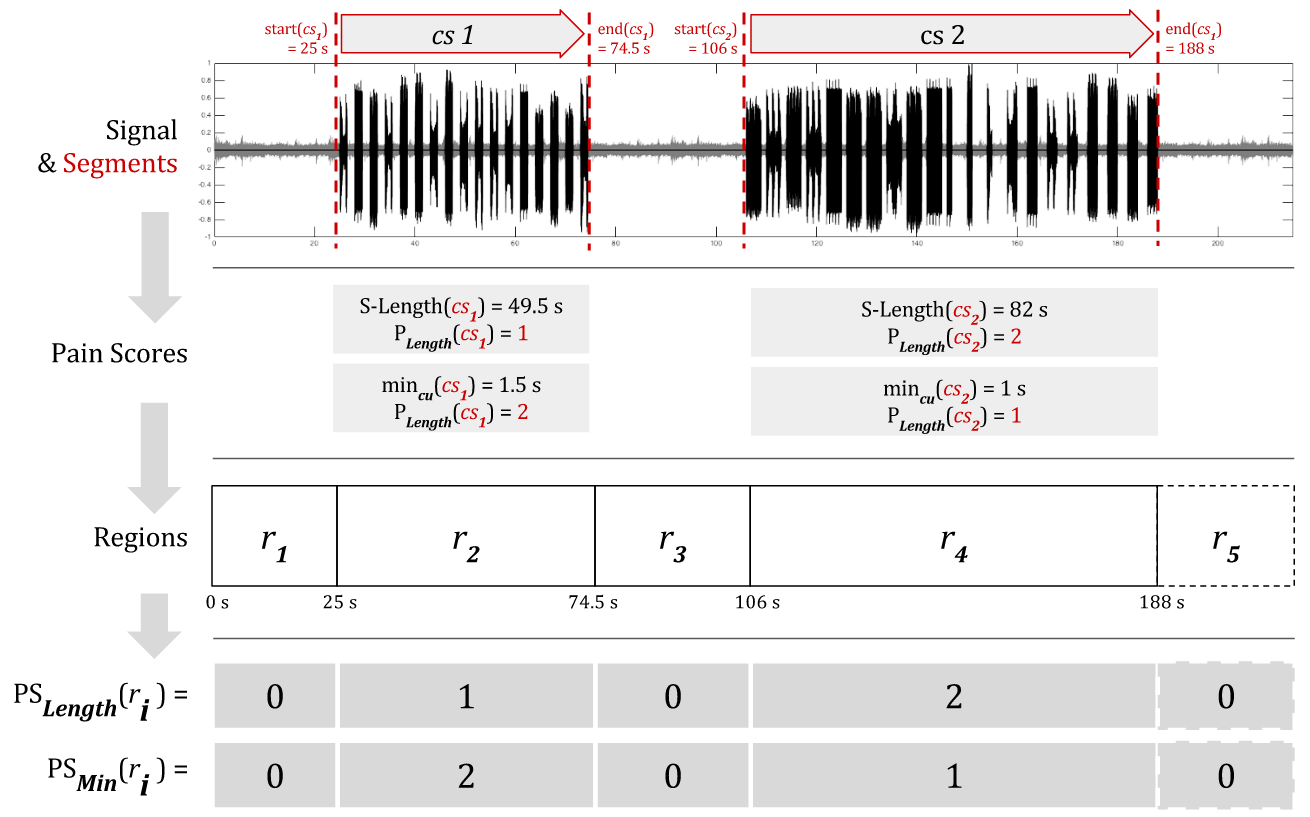
\includegraphics[width=1\textwidth]{bilder/visualisation_example_01.png}
	\caption{Oben: Ein Beispielsignal, sowie zwei Segmente, die mit $t_s = \SI{10}{\second}$ gefunden wurden. Darunter: Pain Scores, die für die beiden Segmente berechnet wurden. Darunter: Schematische Darstellung des Signals als Regionen. Unten: Scores der Regionen.}
	\label{img:visualisation_example_01}
\end{figure}

Die Grundlegende Idee der Visualisierung ist nun, den zeitlichen Verlauf des Signals schematisch als einen \emph{Balken} darzustellen. Dieser Balken wird in \emph{Regionen} eingeteilt. Eine Region $r$ beinhaltet entweder ein Cry-Segment oder den Raum zwischen zwei Cry-Segmenten. Die Länge einer Region entspricht der zeitlichen Länge des jeweiligen Stille- oder Cry-Segmentes. In Abbildung \ref{img:visualisation_example_01} werden fünf Regionen $r_{1} , \ldots , r_5 $ markiert, wobei die Region $r_2$ und $r_4$ Cry-Segmente enthalten. Die letzte Region wurde noch nicht abgeschlossen, da in der Abbildung nur ein Ausschnitt des sich eigentlich noch weiter fortsetzenden Signals gezeigt wird.

Jeder Region wird ein \emph{Region Score} $RS$ nach Formel \ref{eq:region_score} zugewiesen. Beinhaltet eine Region ein Cry-Segment, so wird der Region die entsprechende Pain Score zugewiesen. Beinhaltet die Region kein Cry-Segment, so erhält die Region automatisch einen Score von 0. In Abbildung \ref{img:visualisation_example_01} unten werden die Region Scores für das Beispielsignal nach den beiden fiktiven Pain Scales gezeigt.

\begin{equation}
RS_{\text{Scale}}(r) = \begin{cases}
 0 \quad \quad \quad,  \text{wenn } r  \text{ kein Cry-Segment beinhaltet} \\
 PS_{\text{Scale}}(cs) \;, \text{wenn } r  \text{ ein Cry-Segment } cs \text{ beinhaltet}
 \end{cases}	
 \label{eq:region_score}
\end{equation}

Das Ziel ist es nun, jede Region mit einer Farbe einzufärben, die die Region Score der entsprechenden Region anzeigt. Dazu wird eine Funktion $F_{Scale}:RS \mapsto P_{Scale}$ benötigt, welche in Abhängigkeit von der verwendeten Pain Scale eines Region Score auf eine Farbe abbildet. Die Abbildungsfunktion $F_{Scale}$ wird in diesem Zusammenhang als \emph{Farbschema} bezeichnet und der Funktionsbereich $P_{Scale}$ als \emph{Farbpalette}. Das Farbschema und die Farbpalette soll die folgenden Kriterien erfüllen.

\begin{description}
\item[Diskrete Farbpalette] Die Scores aller in Kapitel \ref{sec:painScores} vorgestellten Pain Scales haben diskrete Wertebereich. Ebenso soll $P_{Scale}$ eine diskrete Menge an Farben enthalten, so dass $|RS_{Scale}| \leq |P_{Scale}|$.
\item[Kleinst mögliche Veränderung des Farbschemas bei Wechsel der Pain Scale] Wird zur Schmerzdiagnostik die Pain Scale verwendet, soll das Farbschema von der alten Pain Scale verwendete Farbschema möglichst einfach auf die neue Pain Scale übertragbar sein. Verwenden zwei Pain Scales den selben Wertebereich bezüglich der Scores, soll das selbe Farbschema verwendet werden. Wird angenommen, dass der geringste Pain Score jeder Pain Scale 0 beträgt\footnote{Die Pain Scale N-PASS bildet hier eine Ausnahme, da sie die Pain Score -2 und -1 definiert. Da diese jedoch die den Grad der Beruhigung diagnostizieren, können sie nur durch die manuelle Zuführung eines Schmerzstimulus festgestellt werden.}, so soll $P_{Scale}$ allein abhängig von dem maximalen Score der jeweiligen Scale sein. 
\item[Intuitive Farbsemantik durch Ampelschema] Das Farbschema soll eine intuitive Zuordnung zwischen der Höhe des Score und der jeweiligen Farbe ermöglichen. In dieser Arbeit wurde sich für ein Ampelschema entschieden. Das heißt, dass der niedrigste Score \glqq grün\grqq{}, der höchst Score \glqq rot\grqq{} und ein \glqq mittelerer\grqq{} Score \glqq gelb\grqq{} dargestellt werden soll. Definiert eine Pain Scale einen maximalen Score von 2, so wie beispielsweise das FLACC-System, so ergibt sich die Abbildung $0 \mapsto $grün, $1 \mapsto $ gelb, $2 \mapsto $ rot. Hat die Pain Scale mehr Scores, wie beispielsweise das MBPS mit ingesamt fünf möglichen Scores, so müssen geeignete Zwischenfarben definiert werden.
\item[Visuelle Gleichabständigkeit der Farben] Pain Scales definieren definieren die Scores zwar in einer Reihenfolge, gewährleisten aber keine Vergleichbarkeit. Das heißt, dass bei beiner Pain Scale ein Score von 4 in jedem Fall schlimmer ist als ein Score von 2, jedoch , das jedoch nicht heißt, dass ein Score von 4 automatisch doppelt so schlimm ist wie ein Score von 2. Die Farben eines Farbschemas sollen eine visuelle Gleichabständigkeit gewährleisten. Das heißt, dass die Farben, auf die zwei auf einander folgende Scores einer Scale abgebildet werden, visuelle den Gleichen abstand zueinander haben. So wird verhindert, dass ein Farbschema eine Nähe oder einen Abstand zweier Scores suggeriert, der durch die Pain Scale nicht vorhanden ist. 
\item[Visuelle Gleichwichtigkeit der Farben] Es kann nicht davon ausgegangen werden, dass ein bestimmter Score für die medizinische Fachkraft interessanter ist als andere Scores. Daher soll keine Farbe einer Farbpalette suggerieren, wichtiger als die anderen Farben der Palette zu sein.
\end{description}

Das Kriterium der Gleichabständigkeit legt die Verwendung des \emph{CIELAB}-Raum zur Farbdefinition für die Farbpaletten nahe. Der Farbraum ist in Bezug auf die Menschliche Farbwahrnehmung gleichförmig. Das heißt, dass die euklidische Distanz zwischen zwei Farben ihrer wahrgenommenen Unterschiedlichkeit entsprechen. Da die Farbedifinition im CIELAB-Raum jedoch auf für den Menschen unintuitiven Parametern beruht, wird weiterhin der \emph{LCH}-Raum verwendet, der zylindrischen Transformation des CIELAB-Raumes. Dieser erlaubt die Farbdefinition auf Basis der für den Menschen intuitiveren Parameter \textbf{L}uminance (Luminanz), \textbf{C}hroma (Buntheit) und \textbf{H}ue (Farbton). Dies Erleichtert die Erfüllung der Farbsemantik, da sich die Farben Grün, Gelb und Rot in der H-Dimension in direkter Nachbarschaft befinden. 

zur Zusammenstellung der konkreten Farbpaletten wird das Unterstützungwertkezug von David Johnstone verwendet.\footnote{\url{http://davidjohnstone.net/pages/lch-lab-colour-gradient-picker}} Das Tool erlaubt die Wahl von $n$ Farben LCH-Raum, bezeichnet als \glqq Fixpunkte\grqq. Auf Basis dieser Fixpunkte generiert das Tool eine Farbpalette mit $m$ Farben. Der erste und der letzte Fixpunkt definieren die erste und die letzte Farbe der Farbpalette. Ist $n = m$, so entspricht die Farbpalette den definierten Fixpunkten. Ist $m > n$, so interpoliert das Tool zwischen den Fixpunkten, um die Zwischenfarben zu finden. Findet diese Interpolation im LCH-Raum statt, so ist die visuelle Gleichabständigkeit der interpolierten Farben zu den benachbarten Fixpunkten gewährleistet.

Ein \glqq reines Rot \grqq, codiert im RGB-Raum mit $[255,0,0]$, hat im LCH-Raum die Koordinaten $[53,105,40]$. \glqq Reines grün\grqq{} hat die Koordinaten RGB $=[0,255,0]$, was LCH $= [88,120,136]$ entspricht. Das \glqq Leicht rötliche Gelb\grqq{} definiert mit RGB $=[255,240,0] \hat{=}$LCH $= [93,93,99]$. Diese Farben haben im LCH Raum eine unterschiedliche Buntheit, weshalb  sie in einer  Farbpalette eine unterschiedliche Wichtigkeit suggerieren würden. Da wurde der Chroma-Wert aller drei Fixpunkte auf den niedrigsten der drei Werte, $93$, gesetzt. Die tatsächlichen Parameter der drei Fixpunkte \emph{Rot}, \emph{Gelb} und \emph{Grün} werden in Tabelle \ref{tab:fixpoints} für den RGB- und den LCH-Farbraum definiert. 

\begin{table}[h]
\centering
\caption{Fixpunkte als Basis der Farbpaletten}
\label{tab:fixpoints}
\begin{tabular}{@{}lllllll@{}}
\toprule
     & \multicolumn{3}{c}{RGB} & \multicolumn{3}{c}{LCH} \\ 
     & R      & G      & B     & L      & C     & H      \\ \midrule
Rot  & 243    & 45     & 22    & 53     & 93    & 40     \\
Gelb & 255    & 240    & 0     & 93     & 93    & 99     \\
Grün & 110    & 250    & 86    & 88     & 93    & 136    \\ \bottomrule
\end{tabular}
\end{table}

Abbildung \ref{fig:color-swatches} zeigt die Farbpaletten, die mit Hilfe des Tools für zwei bis sieben Farben erstellt wurde. Bei der Farbpalette mit ungerader Farbanzahl befinden sich die Fixpunkte an erster, letzter und mittlerer Position, während die zusätzlichen Farben durch Interpolation der benachbarten Farben erzeugt wurden. Bei den Farbpaletten mit gerader Anzahl an Farben ergibt sich das Problem, dass der gelbe Fixpunkt nicht mehr mit enthalten ist.

\begin{figure}[h]
	\centering
	\includegraphics[width=0.75\textwidth]{bilder/colorpics.png}
	\caption{Erstellte Farbpaletten mit 2, 3, 4 und 5 Farben inklusive der zugehörigen RGB-Koordinaten im Hex-Code.}
	\label{fig:color-swatches}
\end{figure}

Auf Basis die Farbpaletten wurden die Farbschemen $P_{Scale}$ definiert, welche die Region-Scores 
